\documentclass[11pt, a4paper]{article} % setsfont size and layout

%% required packages %%

\usepackage[margin=2.5cm]{geometry} % margins
\usepackage[utf8]{inputenc} % Umlaute
\usepackage{amsmath,amssymb, physics}		% math formulas
\usepackage{graphicx}		% graphics
\usepackage{fancyhdr}		% header and footer on every page
\usepackage{setspace}		% line space (e.g. \singlespacing, \onehalfspacing or \doublespacing)

\usepackage{braket}
\usepackage{xcolor}
%% Here the main part of the document begins %%

\begin{document}
	
%% Some more settings %%
	
\setlength{\parindent}{0pt} % first line in paragraph will not be indented
\onehalfspacing				% 1.5 line spacing
%\thispagestyle{empty}		% no header and page number on first page


%% Header on first page with course information etc. %%
%\begin{tabular}{p{15.5cm}}
%	{\large \textbf{Classical Mechanics}} \\
%	Westlake University \\ 
%	\hline
%	\\
%\end{tabular}

\vspace*{0.1cm}				% vertical space between header on top of the page and main heading


\begin{center}
	{\Large \textbf{Classical Mechanics}}
    \vspace*{2mm}
    
    {\Large \textbf{Final Exam}}
	\vspace{8mm}
%Name: 
%\end{center} 
%\vspace{0.1cm}

{\Large \bf \color{red} Time: 2:00 - 4:00 pm, Dec. 30th, 2025}
\vspace*{2mm}

{\Large \bf \color{red} Duration: 120 minutes}
\vspace*{2mm}

{\Large \bf \color{red} Total Points: 100}
\end{center}
\vspace*{8mm}

{\Large \bf \color{orange} Instruction:} 
\vspace*{2mm}

{\Large \bf \color{orange} \hspace{2em} This is a closed-book exam; no aids are allowed.}
\vspace*{2mm}

{\Large \bf \color{orange} \hspace{2em} Total 10 pages including the front page of the instruction.}
\vspace*{2mm}

{\Large \bf \color{orange} \hspace{2em} Provide relevant mathematical steps.} 
\vspace*{2mm}

{\Large \bf \color{orange} \hspace{2em} All answers must be in English.}
\vspace*{2mm}

{\Large \bf \color{orange} \hspace{2em} Don't open the booklet before the exam begins.}
\vspace{5cm}

\begin{center}
{\Large \bf Student Name: \underline{\hbox to 40mm{}}}
\vspace*{8mm}

{\Large \bf Student ID: \underline{\hbox to 40mm{}}}
\vspace*{2mm}
\end{center}

\newpage
\section*{Problem 1 [$5 + 5$ points]} 
\begin{enumerate}
  \item[(1)] Write down Newton’s second law, the Euler-Lagrange equation, and Hamilton’s equations of motion. 

  \item[(2)] Using $S=\int_{t_i}^{t_f}(\dot{q}p-H )\dd t$ and the Least Action Principle to derive the Hamiton's equations of motion.

  \end{enumerate}



\newpage 
\section*{Problem 2 [$10$ points]} 
A particle of mass $m$ is attracted to the origin by a force of magnitude $k/r^2$. Using plane polar coordinates, find the Hamiltonian and Hamilton's equations of motion. Sketch constant-$H$ contours in the $(r,p_r)$ phase plane.

\newpage
\section*{Problem 3 [$10$ points]}
A bead of mass $m$ slides on a frictionless rod inclined at a constant angle $\alpha$ to the vertical axis. The rod rotates about this vertical axis with a constant angular velocity $\omega$. Gravity $g$ acts vertically downwards. Derive the equation of motion for the position $r$ of the bead along the rod using the Lagrangian formalism. 
\begin{figure}[h]
    \centering
    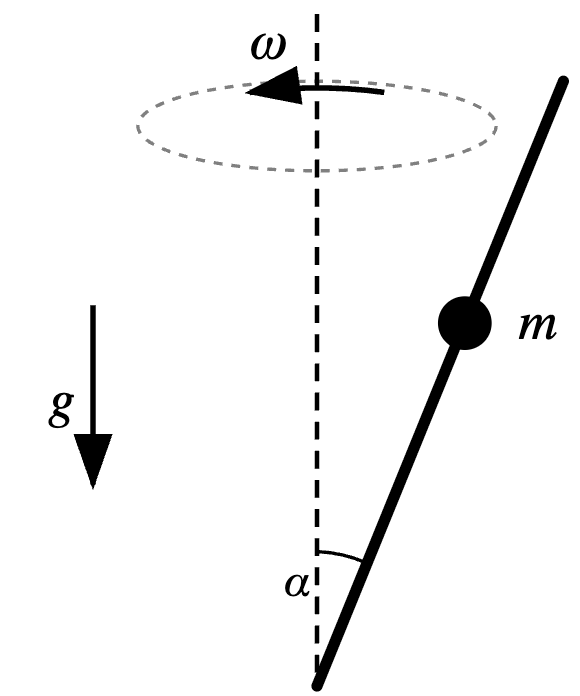
\includegraphics[width=0.35\textwidth]{bead.png}
    \label{P7}
\end{figure}

\newpage
\section*{Problem 4 [$10$ points]}
Consider the simple harmonic oscillator, with a particle of mass $m$ free to move in one dimension, connected to a spring with Hamiltonian

\begin{equation*}
    H = \frac{p^2}{2m} + \frac{1}{2}m\omega^2q^2
\end{equation*}

where $\omega = \sqrt{k/m}$ is the natural angular frequency and $k$ is the spring constant. The phase space is two-dimensional, parameterized by \{$q$, $p$\}. Let us apply the canonical transformation defined as

\begin{equation*}
    F_1(q, Q, t) = qQ.
\end{equation*}

\begin{enumerate}
\item[(1)] Find the new Hamiltonian after the canonical transformation

\item[(2)]  Is following transformation a canonical transformation? Calculate the Poisson bracket to justify your answer. 

\begin{equation*}
    q(Q, P) = \sqrt{\frac{2P}{m\omega}}\sin{Q},\ p(Q, P) = \sqrt{2m\omega P}\cos{Q}.
\end{equation*}
\end{enumerate}

\newpage
\section*{Problem 5 [$10$ points]}
A pendulum consists of a mass $m$ and a massless stick of length $l$. The pendulum support oscillates horizontally with a position given by $x(t) = A \cos(wt)$ (represented by a double-headed arrow in the figure below). What is the general solution for the angle of the pendulum as a function of time?

\begin{figure}[h]
    \centering
    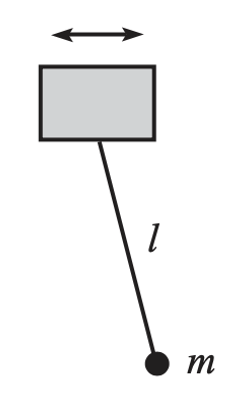
\includegraphics[width=0.25\textwidth]{Finala_P8.png}
    \label{P7}
\end{figure}

% \newpage
% \section*{Problem 6 [$10$ points]}
% Assume $H(q_1, q_2, p_1, p_2)=q_1p_1 -q_2p_2-aq_1^2 + bq_2^2$, where $a$ and $b$ are constants. Calculate the total time derivative of $q_1q_2$.


\newpage
\section*{Problem 6 [$6+6$ points]}
A satellite of mass $m$ carrying a crew is initially in a stable circular orbit (Orbit 1) of radius $R_1$ around a central body of mass $M$. The crew wishes to transfer the satellite to a larger circular orbit (Orbit 3) with a radius of $R_3 = 2R_1$. To achieve this, they perform a maneuver involving two successive impulsive boosts. 
First, the satellite performs an initial boost that increases its velocity instantaneously, placing it onto an elliptical transfer orbit (denoted as Orbit 2). This transfer orbit has its perigee at radius $R_1$ (the radius of the initial circular orbit) and its apogee at $R_3 = 2R_1$.
Next, upon reaching the apogee of the transfer orbit (point $P'$), the satellite performs a second instantaneous velocity change. This second boost increases the satellite's speed such that it transitions into a final circular orbit of radius $2R_1$.
\begin{enumerate}
    \item[(1)] Determine the thrust factor $\lambda$ required for the first boost, defined as the ratio of the speed after the boost to the speed before the boost ($\lambda = v_{p} / v_1$).
    \item[(2)] Determine the thrust factor $\lambda'$ required for the second boost, defined as the ratio of the speed after the boost to the speed before the boost ($\lambda' = v_3 / v_{p'}$).
\end{enumerate}

\textbf{Hint:} The orbit of a satellite is given by $
r(\phi) = \frac{c}{1 + \epsilon \cos \phi}$. 
$\epsilon$ is the eccentricity of the orbit; $c = \frac{L^2}{GMm^2}$, where $L$ is the satellite’s angular momentum.

\begin{figure}[h]
    \centering
    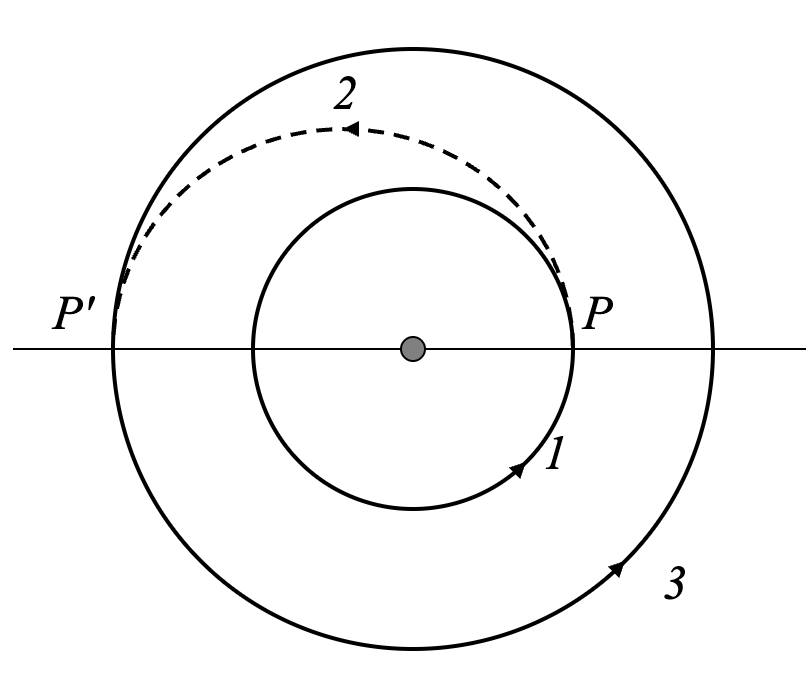
\includegraphics[width=0.3\textwidth]{transfer.png}
    \label{P7}
\end{figure}

% \newpage
% \section*{Problem 5 [$5+5$ points]}
% \begin{enumerate}
% \item[(1)] Prove that the transformation 
% \begin{equation*}
%    Q = p/\tan q
% \end{equation*}
% \begin{equation*}
% P = \ln{\left(\frac{\sin q}{p}\right)}
% \end{equation*}
% is canonical. 
% \item[(2)] Find the generating function $F_1(q, Q)$ for this transformation.
% \end{enumerate}

\newpage
\section*{Problem 7 [$6 + 10$ points]}
\begin{enumerate}
\item[(1)]  What are the conditions on the ``small" constants $a$, $b$, $c$, $d$, $e$, and $f$ in order that 
\begin{equation*}
    q= Q+ aQ^2+2bQP + cP^2
\end{equation*}
\begin{equation*}
   p=P+dQ^2+2eQP+fP^2
\end{equation*}
be canonical transformation to \textbf{first order} in small quantities?

\item[(2)] The Hamiltonian for a slightly anharmonic oscillator is 
\begin{equation*}
   H=\frac{p^2}{2m} + \frac{1}{2}m\omega^2q^2 + \beta q^3
\end{equation*}
where $\beta$ is ``small". Perform a canonical transformation of the type given in (1) and adjust the constants so that the new Hamiltonian $H$ does not contain an anharmonic term to first order in small quantities, thus 
\begin{equation*}
   H'=\frac{P^2}{2m} + \frac{1}{2}m\omega^2Q^2 + ...
\end{equation*}
Write down the transformations rules between $(q, p)$ and $(Q, P)$.
\end{enumerate}

% \newpage
% \section*{Problem 8 [10 points]}
% \hspace{2em} A Hamiltonian with one degree of freedom has the form
% \begin{equation*}
%     H = \frac{p^2}{2m} + \frac{kq^2}{2} - 2aq^3\sin\alpha t
% \end{equation*}
% where $m$, $k$, $a$, and $\alpha$ are constants. Find the Lagrangian corresponding to this Hamiltonian. Write out both Hamilton's equations and Euler-Lagrange equations, and show directly that they are equivalent.
% \end{enumerate}


\newpage
\section*{Problem 8 [$12$ points ]}
Two equal masses $m$, connected by a massless string, hang over two pulleys (of negligible size), as shown in the Figure below. The left one moves in a vertical line, but the right one is free to swing back and forth in the plane of the masses and pulleys. Find the equations of motion for $r$ and $\theta$, as shown.


\begin{figure}[h]
    \centering
    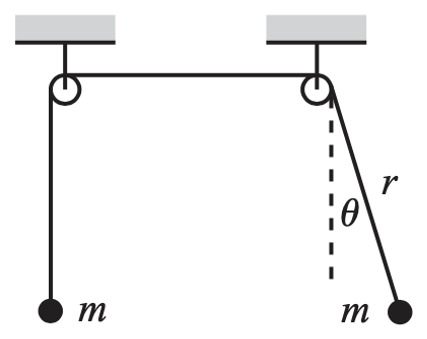
\includegraphics[width=0.4\textwidth]{Finala_P9.png}
    \label{P7}
\end{figure}

\newpage
\section*{Problem 9 [$10$ points]}
Consider a particle of mass $m$ and electric charge $q$ moving in the presence of time-dependent electromagnetic fields. The particle's motion is described by the relativistic Lagrangian:
\[
L = -mc^2\sqrt{1 - \frac{v^2}{c^2}} + q\, \mathbf{v} \cdot \mathbf{A}(\mathbf{r}, t) - q\, V(\mathbf{r}, t),
\]
where $\mathbf{v} = \dv{\mathbf{r}}{t}$ is the particle's velocity; $V(\mathbf{r}, t)$ is the scalar potential; $\mathbf{A}(\mathbf{r}, t)$ is the vector potential; $c$ is the speed of light. Take the non-relativistic limit by expanding the Lagrangian to leading order in $v/c$ (i.e., assume $v \ll c$). From the resulting approximate Lagrangian, derive the Hamilton's equations of motion.
Hint: $\mathbf{E} = -\nabla V - \pdv{\mathbf{A}}{t}$ and $\mathbf{B} = \nabla \times \mathbf{A}$.



\end{document}